\section{Robust solution}

Beamforming techniques for sound localization have been study intensively over the last decades. The main drawback of the conventional beamforming are the side lobes in the localization results. If SRP-PHAT algorithm is applied to a tetrahedral array and cross-correlations values at different delays are summed by the beamformer (Eq. \ref{eq:srpSum}), subsidiary peaks can appear in the energy map at DOAs that don't correspond to the incident plane wave DOA. Those peaks in the SRP-PHAT energy map can mask real sources or even add up to other peaks from other sources, thus display a fake source. Deconvolution methods remove those peaks to reveal the correct peak. The algorithms for deconvolution are based on the point spread function, which is the response of the array to a point source. For far-field, this means a plane wave incident with a particular DOA on the microphone array. In transfer function terms, the array response is `deconvolved' from the final energy map. While this problem has motivated the creation of new beamformers {!!CITATION!!}, the problem lies in the method itself. New classes of algorithms has been developed to deconvolve the noise signals from the desired steered signal such as CLEAN \cite{sijtsma2007clean}. Even if CLEAN was applied successfully, it was in 2006 that the deconvolution approach for the mapping of acoustic sources (DAMAS) was proposed \cite{brooks2006deconvolution} and was acknowledged a major breakthrough in array processing. At first research was mainly focused on aeroacoustic for the development of near-field sound localization system but it seems that a new enthusiasm has taken over scientists trying to solve other sound localization problems. While the DAMAS method is mainly designed for near field measurements in the range of the array aperture size, a new method is proposed in \cite{zhao2015large} and \cite{zhao2017large} where a small aperture array is used to measure source signal in the far field. The principle behind point spread function is discussed in the following section. Then a review of the underlying principles of the main deconvolution algorithms is given, and finally a specific method for coherent and incoherent sources localization is discussed.

\subsection{Point spread function}
Point spread function is the response of an `imaging' system to a point source. In the context of sound localization, this is the loci of point sound source detected by the microphone array. A perfect array will detect a point precisely at the actual source location and nothing elsewhere. This, however, is not the general case. For example, given a single pair of microphones, and assuming far-field incidence, the only information that can be concluded from a single point source is the angle of incidence on the array. This angle is a vector combination of source azimuth and elevation. This leads to a circle around the array where the source might be located (circular maximum peak). This circle is the base of the cone resulting from the cone approximation discussed previously.

%\begin{figure}[H]
%    \centering
%    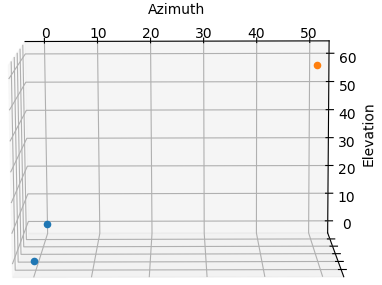
\includegraphics[width=0.98\textwidth]{Figures/2mic1src.png}
%    \caption{Figure depicts a source located at $50\degree$ azimuth and $60\degree$ elevation (orange dot). Two microphones (blue dots) will be used to localize the source.}
%    \label{fig:2mic1srcPos}
%\end{figure}

\begin{figure}[H]
    \centering
    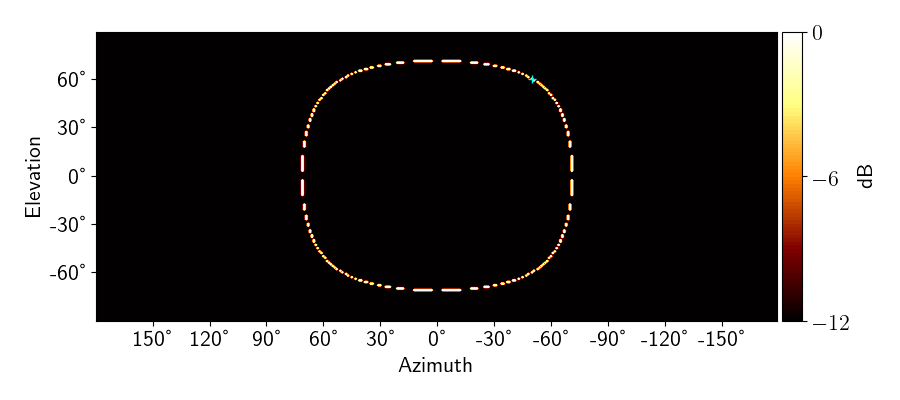
\includegraphics[width=0.98\textwidth]{Figures/2mic1srcRes.png}
    \caption{SRP-PHAT is run to localize the source. As expected the source is localized to a circle. The red dot indicates the actual source location.}
    \label{fig:2mic1src}
\end{figure}

If three microphones are placed in a horizontal equilateral triangle, we get three circles (three possible pairs of microphones) from localization. The maximum peak occurs at 2 locations with azimuth=50$\degree$ and elevation=$\pm 60\degree$.
\begin{figure}[H]
    \centering
    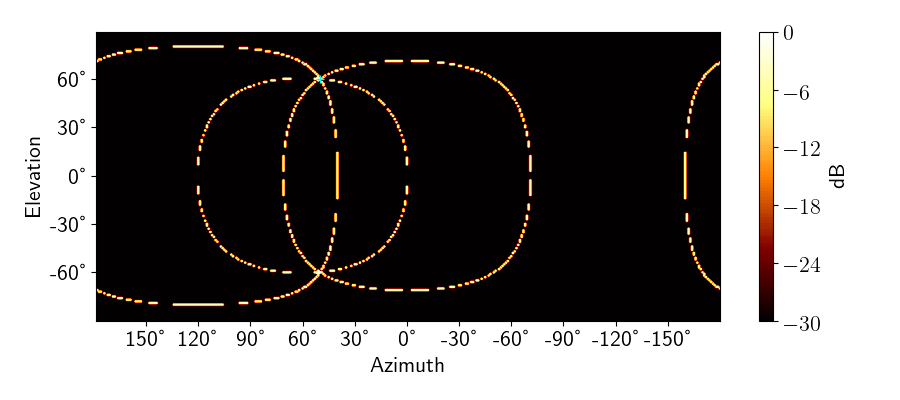
\includegraphics[width=0.98\textwidth]{Figures/3mic1srcRes.png}
    \caption{SRP-PHAT is run to localize the source with 3 microphones.}
    \label{fig:3mic1src}
\end{figure}

For a tetrahedral array, the point spread function is a combination of circles from the 6 possible microphone pairs. This time the main peak occurs at exactly one point. 
\begin{figure}[H]
    \centering
    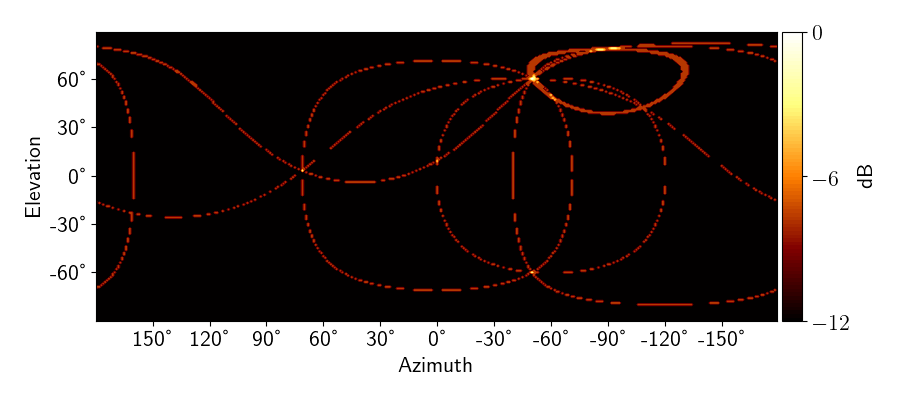
\includegraphics[width=0.98\textwidth]{Figures/4mic1srcRes.png}
    \caption{SRP-PHAT is run to localize the source with a tetrahedral array.}
    \label{fig:4mic1src}
\end{figure}

The result in fig.\ref{fig:4mic1src} is applicable only in ideal conditions (zero noise, no reflections and perfectly planar propagation). In noisy conditions, the localization result is depicted in fig. \ref{fig:4mic1srcNoisy}. Note that the color bars for the figures depicted are of the same color scale. The localization performance deteriorates as the SNR drops. The result is similar to the results for PHAT with 2 microphones discussed earlier as the underlying process in SRP-PHAT is still PHAT. 

As can be seen in Fig. \ref{fig:4mic1src}, even in ideal conditions, the localization results contain many peaks of varying heights. This is due to summing the cross-correlation responses of a non-linear array (Eq. \ref{eq:srpSum}). If the array were linear, the localization circles from each pair would all overlap completely. In case of a tetrahedral array, the localization circles from the possible microphone pairs are not co-planar. This is because all the edges of a tetrahedron point in the different directions. The obvious problem here is multi-source detection. If multiple sources are playing at different levels, how do we determine if the detected peak is a source or a relic from another higher level source? The methods to do so form the basis of deconvolution methods. 
A simple deconvolution approach could be to penalize sources detected only by a subset of the microphone pair combinations. This could be done by taking a product and not a sum in Eq. \ref{eq:srpSum}. This way, if a peak is caused by a single localization circle, the cross-correlation values from other microphone pairs would be close to zero, and thus would scale the false peak down. The localization results from this are given in fig. \ref{fig:4mic1srcNoisyProd}. Fig. \ref{fig:4mic2srcNoisyCompare} compares the localization result for two equally loud sources, this time located at (azimuth, elevation) = (-20, -30) and (50, 60), with summed SRP-PHAT and product-SRP-PHAT. The results are convincingly better, atleast for simulations.  

\begin{figure}[H]
    \centering
    \begin{subfigure}[b]{0.96\textwidth}
    \centering
    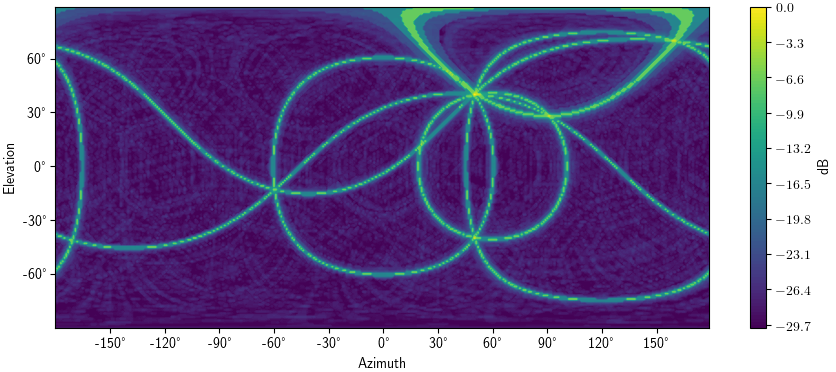
\includegraphics[width=0.8\textwidth]{Figures/4mic1src20.png}
\end{subfigure}
\vskip \baselineskip
\begin{subfigure}[b]{0.96\textwidth}
    \centering
    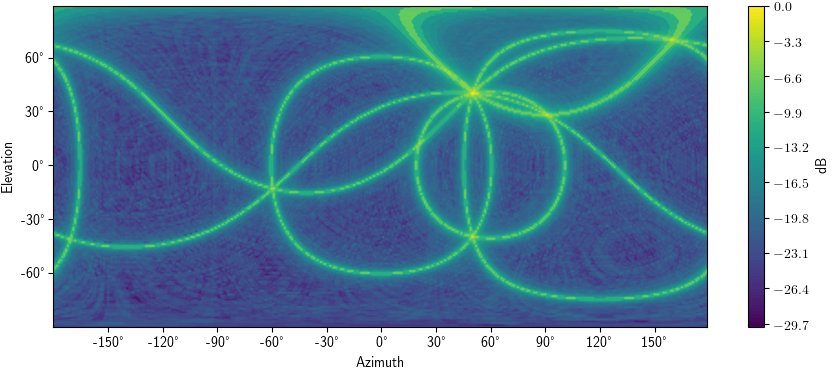
\includegraphics[width=0.8\textwidth]{Figures/4mic1src6.png}
\end{subfigure}
\vskip \baselineskip
\begin{subfigure}[b]{0.96\textwidth}
    \centering
    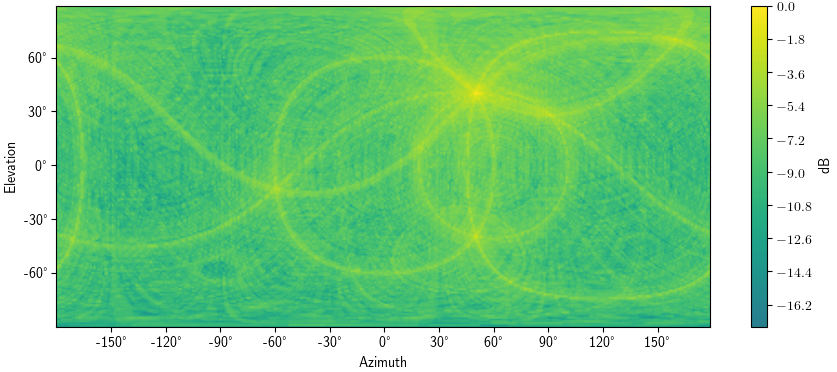
\includegraphics[width=0.8\textwidth]{Figures/4mic1src0.png}
\end{subfigure}
\vskip \baselineskip
\begin{subfigure}[b]{0.96\textwidth}
    \centering
    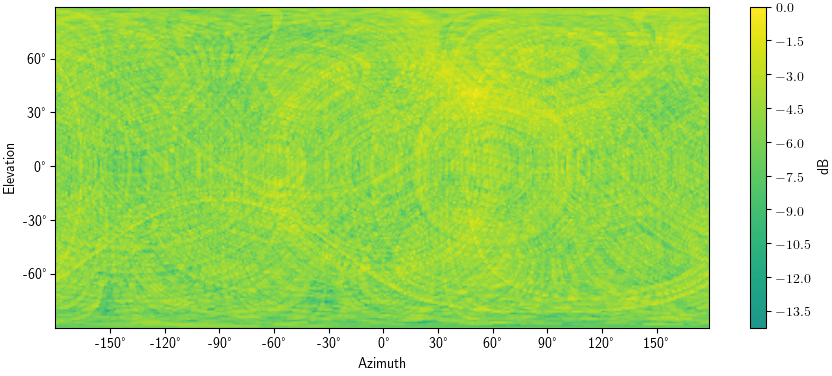
\includegraphics[width=0.8\textwidth]{Figures/4mic1srcNeg6.png}
\end{subfigure}
\caption{Figures depict from top-to-bottom SRP-PHAT localization results with SNR = 20dB, SNR = 6dB, SNR = 0dB, SNR = -6dB}
\label{fig:4mic1srcNoisy}
\end{figure}

 \begin{figure}[H]
    \centering
    \begin{subfigure}[b]{0.96\textwidth}
    \centering
    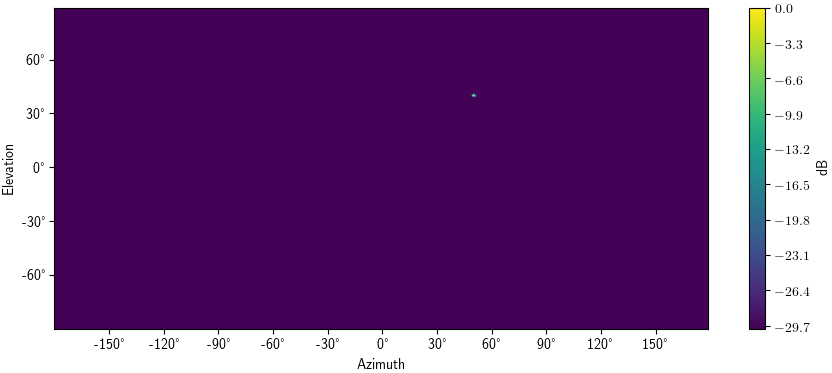
\includegraphics[width=0.8\textwidth]{Figures/4mic1src20Prod.png}
\end{subfigure}
\vskip \baselineskip
\begin{subfigure}[b]{0.96\textwidth}
    \centering
    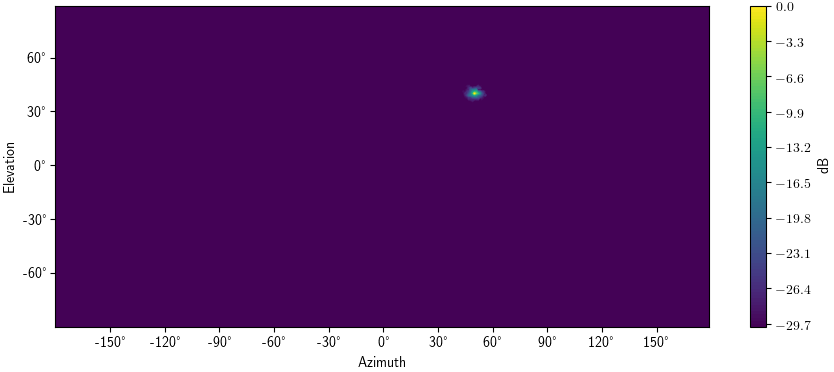
\includegraphics[width=0.8\textwidth]{Figures/4mic1src6Prod.png}
\end{subfigure}
\vskip \baselineskip
\begin{subfigure}[b]{0.96\textwidth}
    \centering
    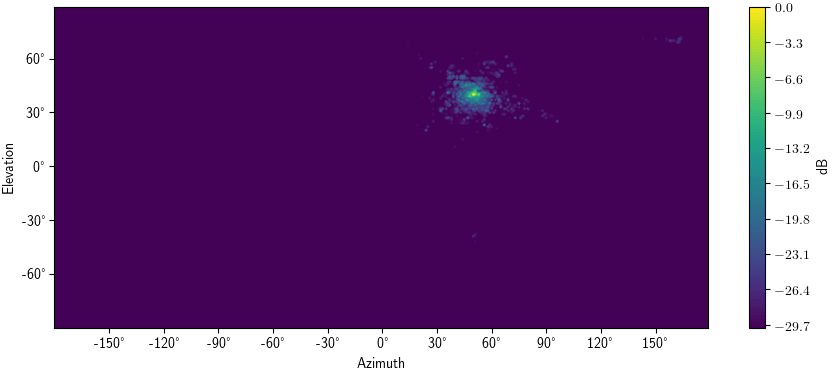
\includegraphics[width=0.8\textwidth]{Figures/4mic1src0Prod.png}
\end{subfigure}
\vskip \baselineskip
\begin{subfigure}[b]{0.96\textwidth}
    \centering
    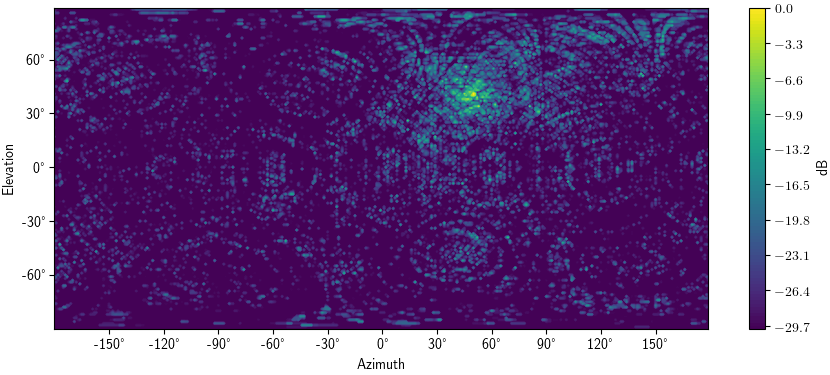
\includegraphics[width=0.8\textwidth]{Figures/4mic1srcNeg6Prod.png}
\end{subfigure}
\caption{Figures depict from top-to-bottom product-SRP-PHAT localization results  with SNR = 20dB, SNR = 6dB, SNR = 0dB, SNR = -6dB}
\label{fig:4mic1srcNoisyProd}
\end{figure}

 \begin{figure}[H]
    \centering
    \begin{subfigure}[b]{0.96\textwidth}
    \centering
    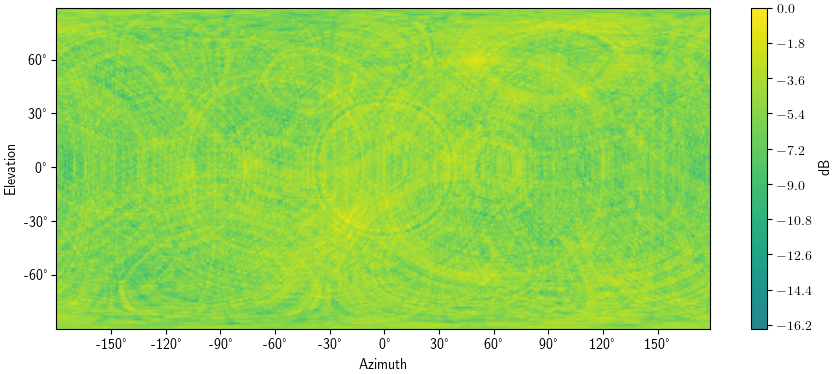
\includegraphics[width=0.8\textwidth]{Figures/4mic2srcNeg6Sum.png}
\end{subfigure}
\vskip \baselineskip
\begin{subfigure}[b]{0.96\textwidth}
    \centering
    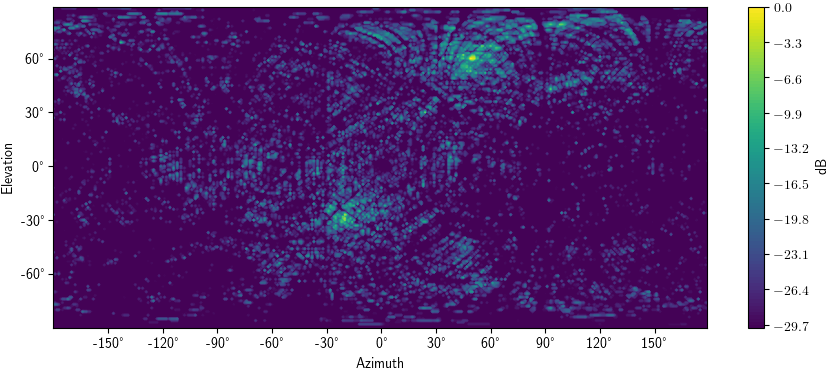
\includegraphics[width=0.8\textwidth]{Figures/4mic2srcNeg6Prod.png}
\end{subfigure}
\caption{Figures depict from localization results with summed-SRP-PHAT (top) and product-SRP-PHAT (bottom)}
\label{fig:4mic2srcNoisyCompare}
\end{figure}

The drawback of using product-SRP-PHAT is that the sound level difference between the different sound sources is lost. In summed-SRP-PHAT, the array magnitude response at a particular azimuth and elevation could be averaged over all microphone pair combinations. Then the level difference between 2 sources is maintained. In product-SRP-PHAT this would not be the case. However if it is assumed that a particular source will have similar magnitude response for all microphone pairs (which is not a strong assumption in far-field), then taking the root ($6^{th}$ root for a tetrahedral array) of the responses, the level difference can be maintained. When plotted on dB scale, that means a simple division by 6, which can be a disadvantage as can be seen in fig. \ref{4mic2srcNoisyDiv}.

\begin{figure}[h]
    \centering
    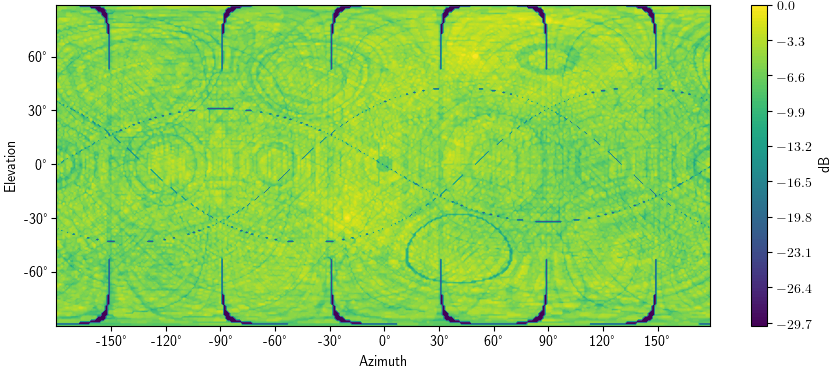
\includegraphics[width=0.98\textwidth]{Figures/4mic2srcNeg6ProdDiv.png}
    \caption{Product-SRP-PHAT is run to localize 2 sources located at (azimuth, elevation) = (-20, -30) and (50, 60) with a tetrahedral array. The result is divided by 6 and normalized before visualization to maintain the level difference between the different sources.}
    \label{fig:4mic2srcNoisyDiv}
\end{figure}